\documentclass[11pt]{article}           
\usepackage[UTF8]{ctex}
\usepackage[a4paper]{geometry}
\geometry{left=2.0cm,right=2.0cm,top=2.5cm,bottom=2.25cm}

\usepackage{xcolor}
\usepackage{paralist}
\usepackage{enumitem}
\setenumerate[1]{itemsep=1pt,partopsep=0pt,parsep=0pt,topsep=0pt}
\setitemize[1]{itemsep=0pt,partopsep=0pt,parsep=0pt,topsep=0pt}
\usepackage{comment}
\usepackage{booktabs}
\usepackage{graphicx}
\usepackage{float}
\usepackage{sgame} % For Game Theory Matrices 
% \usepackage{diagbox} % Conflict with sgame
\usepackage{amsmath,amsfonts,graphicx,amssymb,bm,amsthm}
%\usepackage{algorithm,algorithmicx}
\usepackage{algorithm,algorithmicx}
\usepackage[noend]{algpseudocode}
\usepackage{fancyhdr}
\usepackage{tikz}
\usepackage{pgfplots}
\pgfplotsset{compat=1.18}
\usepackage{graphicx}
\usetikzlibrary{arrows,automata}
\usepackage[hidelinks,colorlinks, citecolor=blue]{hyperref}
\usepackage{extarrows}
\usepackage{totcount}
\setlength{\headheight}{14pt}
\setlength{\parindent}{0 in}
\setlength{\parskip}{0.5 em}
\usepackage{helvet}
\usepackage{dsfont}
% \usepackage{newtxmath}
\usepackage[labelfont=bf]{caption}
\renewcommand{\figurename}{Figure}
\usepackage{lastpage}
\usepackage{istgame}
\usepackage{cleveref}
\crefname{figure}{\textbf{Figure}}{Figures}
\crefname{table}{\textbf{Table}}{Tables}
\usepackage{tcolorbox}
\usepackage{minted}
\usepackage{multirow}

\renewcommand{\tablename}{Table}

\definecolor{LightGray}{gray}{0.9}
\setminted{autogobble = true, baselinestretch = 0.9, beameroverlays = on, escapeinside=||}

% \setlength\partopsep{0pt}
% \setlength\topsep{0pt}
\setlength\parskip{0pt}
% \setlength\itemsep{0pt}
% \setlength\parsep{0pt}
% \setlength{\belowcaptionskip}{0pt}
% \setlength{\abovecaptionskip}{0pt}
% \setlength{\intextsep}{0pt}
% \setlength{\textfloatsep}{0pt}
% \setlength{\floatsep}{0pt}

% \newdateformat{mydate}{\shortmonthname[\THEMONTH]. \THEDAY \THEYEAR}

\RequirePackage{algorithm}

\makeatletter
\newenvironment{algo}
  {% \begin{breakablealgorithm}
    \begin{center}
      \refstepcounter{algorithm}% New algorithm
      \hrule height.8pt depth0pt \kern2pt% \@fs@pre for \@fs@ruled
      \parskip 0pt
      \renewcommand{\caption}[2][\relax]{% Make a new \caption
        {\raggedright\textbf{\fname@algorithm~\thealgorithm} ##2\par}%
        \ifx\relax##1\relax % #1 is \relax
          \addcontentsline{loa}{algorithm}{\protect\numberline{\thealgorithm}##2}%
        \else % #1 is not \relax
          \addcontentsline{loa}{algorithm}{\protect\numberline{\thealgorithm}##1}%
        \fi
        \kern2pt\hrule\kern2pt
     }
  }
  {% \end{breakablealgorithm}
     \kern2pt\hrule\relax% \@fs@post for \@fs@ruled
   \end{center}
  }
\makeatother

\renewcommand{\refname}{References}

\newtheorem{theorem}{Theorem}
\newtheorem{lemma}[theorem]{Lemma}
\newtheorem{proposition}[theorem]{Proposition}
\newtheorem{claim}[theorem]{Claim}
\newtheorem{corollary}[theorem]{Corollary}
\newtheorem{definition}[theorem]{Definition}
\newtheorem*{definition*}{Definition}

\newenvironment{problem}[2][Problem]{\begin{trivlist}
    \item[\hskip \labelsep {\bfseries #1}\hskip \labelsep {\bfseries #2.}]\songti}{\hfill$\blacktriangleleft$\end{trivlist}}
\newenvironment{answer}[1][Solution]{\begin{trivlist}
    \item[\hskip \labelsep {\bfseries #1.}\hskip \labelsep]}{\hfill$\lhd$\end{trivlist}}

\newcommand\1{\mathds{1}}
% \newcommand\1{\mathbf{1}}
\newcommand\R{\mathbb{R}}
\newcommand\E{\mathbb{E}}
\newcommand\N{\mathbb{N}}
\newcommand\NN{\mathcal{N}}
\newcommand\per{\mathrm{per}}
\newcommand\PP{\mathbb{P}}
\newcommand\dd{\mathrm{d}}
\newcommand\ReLU{\mathrm{ReLU}}
\newcommand{\Exp}{\mathrm{Exp}}
\newcommand{\arrp}{\xrightarrow{P}}
\newcommand{\arrd}{\xrightarrow{d}}
\newcommand{\arras}{\xrightarrow{a.s.}}
\newcommand{\arri}{\xrightarrow{n\rightarrow\infty}}
\newcommand{\iid}{\overset{\text{i.i.d}}{\sim}}

% New math operators
\DeclareMathOperator{\sgn}{sgn}
\DeclareMathOperator{\diag}{diag}
\DeclareMathOperator{\rank}{rank}
\DeclareMathOperator{\tr}{tr}
\DeclareMathOperator{\Var}{Var}
\DeclareMathOperator{\Cov}{Cov}
\DeclareMathOperator{\Corr}{Corr}
\DeclareMathOperator{\MSE}{MSE}
\DeclareMathOperator{\Bias}{Bias}
\DeclareMathOperator*{\argmax}{argmax}
\DeclareMathOperator*{\argmin}{argmin}


\definecolor{lightgray}{gray}{0.75}


\begin{document}

\pagestyle{fancy}
\lhead{\CJKfamily{zhkai} 北京大学}
\chead{}
\rhead{\CJKfamily{zhkai} 2025年春\ 几何计算前沿(王鹏帅)}
\fancyfoot[R]{} 
\fancyfoot[C]{\thepage\ /\ \pageref{LastPage} \\ \textcolor{lightgray}{最后编译时间: \today}}


\begin{center}
    {\LARGE \bf Final Project: 3D Latent Diffusion Generation} 

    {\kaishu 姓名:方嘉聪\ \  学号: 2200017849}            % Write down your name and ID here.
\end{center}

\section{Introduction}
\subsection{整体介绍}
参考 SDFusion~\cite{cheng2023sdfusion}, 先预训练 VQ-VAE, 而后是基于 Diffusion Generation 实现了 latent space 下的无条件生成与文本条件生成, 具体见下:
\begin{itemize}
    \item VQ-VAE 使用 ShapeNet~\cite{shapenet} 中 \texttt{chair}, \texttt{rifle}, \texttt{table}, \texttt{sofa} 和 \texttt{speaker} 5类物体进行训练, 重建结果~\cref{fig:reconstruction_vqvae}, 可以基本重建出物体的形状.
    \item 基于VQ-VAE, 在前4类物体数据上分别训练了 U-Net 用于无条件生成, 结果见~\cref{fig:chairs_table_unconditional,fig:sofa_rifle_unconditional}.
    \item 对于文本条件生成, 使用 Text2Shape~\cite{chen2018text2shape} 数据集和预训练的文本编码器(T5-Base~\cite{2020t5}), 
    支持文本控制 \texttt{chair} 和 \texttt{table} 的生成,结果见~\cref{fig:conditional_text_1,fig:conditional_text_2}. 
\end{itemize}
\subsection{项目结构}
整个项目结构如下:
\begin{itemize}
    \item \texttt{data/} 与 \texttt{dataset\_info\_files/}: 数据集与数据集的元数据文件, 由于数据集较大, 可以参照 \texttt{README.md} 进行下载和预处理 (需要一定的时间).
    \item \texttt{vqvae/}: VQ-VAE 模型的实现.
    \item \texttt{diffusion\_unet}: U-Net 模型的实现.
    \item \texttt{test\_*.py} 与 \texttt{train\_*.py}: 训练与测试脚本, 分别对应 VQ-VAE 和 U-Net 的训练与测试.
    \item \texttt{results/}: 生成结果的保存目录, 以 \texttt{.obj} 保存, 报告中的图片均来自该目录下的结果, 使用 MeshLab 可视化并截图.
    \item \texttt{log\_weights/}: 训练过程中保存的模型权重及日志文件, 以便后续分析与复现. 由于模型较大, 可以从 \href{https://disk.pku.edu.cn/link/AA3B115F519B354D259577EF3575C34B2A}{北大网盘} 下载, 解压后放置在根目录即可. 
    \item \texttt{doc/}: 文档目录, 包含本报告的 LaTeX 源文件和结果截图(\texttt{doc/imgs/}).
\end{itemize}

\section{Methods}
整体的框架见~\cref{fig:pipeline}, 与 SDFusion~\cite{cheng2023sdfusion} 的训练与测试流程类似, 模型具体架构与实现上由于算力和时间限制进行了调整, 具体见下:

\begin{figure}[htbp]
    \centering
    \includegraphics[width=0.8\textwidth]{imgs/SDFusion_Arch.png}
    \caption{The overall pipeline of the project. The VQ-VAE is trained first, then the diffusion model is trained for unconditional and conditional 3D generation. The pipeline image is from SDFusion~\cite{cheng2023sdfusion}.}
    \label{fig:pipeline}
\end{figure}
\subsection{VQ-VAE}
鉴于 VQ-VAE~\cite{VQ-VAE} 是经典的生成模型, 本次项目没有重新实现, 在网络架构上与 SDFusion相同, 在\texttt{chair}, \texttt{rifle}, \texttt{table}, \texttt{sofa} 和 \texttt{speaker} 5类物体进行训练\footnote{没有使用 \texttt{car} 类别是因为数据文件大小过大, 上传到机器上需要较长时间.}. 
记编码器和解码器分别为 $E_\phi, D_{\tau}$, 输入的 T-SDF $\mathbf{X} \in \R^{64\times 64 \times 64}$ (T-SDF 阈值为 $0.2$), 那么
\begin{equation}
    \mathbf{z} = E_\phi(\mathbf{X}), \quad \hat{\mathbf{X}} = D_\tau(\text{VQ}(\mathbf{z}))
\end{equation}
在实际训练中令 $\mathbf{z} \in \R^{16\times 16\times 16}$. 损失函数与 VQ-VAE 相同, 即
\begin{equation}
    \mathcal{L}_{\text{VQ-VAE}} = -\log p(\mathbf{X}|\mathbf{z}) + \|\text{sg}[\text{VQ}(\mathbf{z})] - \mathbf{z}\|^2 + \|\text{VQ}(\mathbf{z}) - \text{sg}[\mathbf{z}]\|^2
\end{equation}
其中 $\text{sg}[\cdot]$ 表示停止梯度传播(stop gradient).

\begin{figure}[htbp]
    \centering
    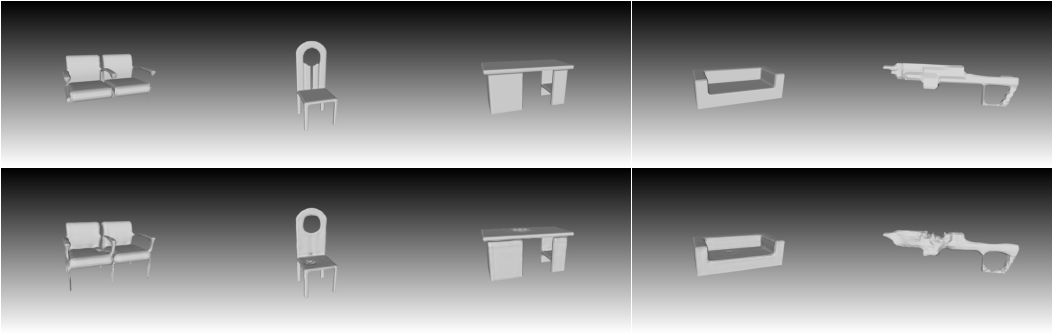
\includegraphics[width=1.0\textwidth]{imgs/vqvae.pdf}
    \caption{The reconstruction results of VQ-VAE on the test set of ShapeNet. The first row is the original object, the second row is the reconstructed object.}
    \label{fig:reconstruction_vqvae}
\end{figure}

在训练完成后从测试集中随机采样 SDF 作为输入, 经过 VQ-VAE 重建之后的结果见 \cref{fig:reconstruction_vqvae}. VQ-VAE 能够重建出大多数细节, 但是对于一些细节会有损失, 特别是对于\texttt{rifle}这类相对较小的物体. 
此外还注意到生成的\texttt{table}会有一个凹陷处 (第三列), 没有弄清产生的原因. 在后续生成的结果中同样有部分结果有这一凹陷, 猜测还是由于 VQ-VAE 重建的信息损失导致的.

\subsection{Unconditional Generation}
\paragraph{模型架构.} 对于无条件的生成, 在~\cite{unet-3d} 的基础上进行修改, 基于 \texttt{ResidualUNet3D} 模块(未添加 Attention Module) 实现了 UNet-Diffusion Model, 添加了必要的 time embedding 模块, 采样 scheduler 使用最简单的 DDPM.
最终使用的模型配置为:
\begin{minted}[bgcolor=LightGray]{python}
    "medium": {
            "time_emb_dim": 256,
            "f_maps": 128,
            "num_levels": 3,
        },
\end{minted}
更细节的实现可以参考 \texttt{./diffusion\_unet/model.py} 与 \texttt{./train\_unet.py}, 可以通过训练脚本的命令行参数修改模型的大小. 

\paragraph{优化目标.} 在训练时, 给定任意一个 input latent $\mathbf{z}$, $\mathbf{z}_t$ 为向$\mathbf{z}$添加 $t$ 步高斯噪声 $\epsilon \in \mathcal{N}(0,1)$ 后的结果
U-Net $\epsilon_\phi$ 的优化目标为
\begin{equation}
    \mathcal{L}_{\text{simple}} := \E_{\mathbf{z}, \epsilon \in \mathcal{N}(0,1)} \left[\|\epsilon - \epsilon_{\phi}(\mathbf{z_t}, t)\|^2\right]
\end{equation}
\paragraph{测试.} 随机从高斯噪声中采样 $\mathbf{z'} \in \R^{16\times 16\times 16}$, 经过 $\epsilon$ 去噪与 $D_\tau$ 解码后即可得到最终的 SDF.

\subsection{Text Conditioned Generation}
\paragraph{模型架构.} 参考了 SDFusion~\cite{cheng2023sdfusion} 中的一些基础模块, 相较于无条件生成, 向 U-Net 中添加了 Self-Attention 和 Cross-Attention 模块.
分为 Downsample Block, Middle Block 和 Upsample Block 三个部分, 其中 Downsample Block 和 Upsample Block 中每一次降采样 \texttt{num\_res\_blocks} 设置为 2, 在制定的层数上添加了 Cross-Attention 模块, 具体见 \texttt{./diffusion\_unet/model\_attention.py}.

文本编码器选择了 Google 的 T5-Base~\cite{2020t5}, 通过 Hugging Face \texttt{transformers} 库下载与调用. 输入的控制文本通过 T5 编码器编码为 text embedding 后, 
通过 Cross-Attention 模块添加进 U-Net 中, 控制扩散过程. 注意这里与 SDFusion 不同, 没有将 text embedding 拼接到 input latent 上\footnote{在实现早期遗漏了 SDFusion 的这一点, 测试结果发现已经达到预期, 没有再修改重新训练.}.

\paragraph{优化目标.} 在训练时, 给定任意一个 input latent $\mathbf{z}$ 和对应的描述文本 $c$, 设文本编码器为 $T_\theta$, $\mathbf{z}_t$ 为向$\mathbf{z}$添加 $t$ 步高斯噪声 $\epsilon \in \mathcal{N}(0,1)$ 的结果, 那么 U-Net $\epsilon_\phi$ 的优化目标为
\begin{equation}
    \mathcal{L}_{\text{text}} := \E_{\mathbf{z}, \epsilon \in \mathcal{N}(0,1)} \left[\|\epsilon - \epsilon_{\phi}(\mathbf{z_t}, t, T_\theta(c))\|^2\right]
\end{equation}
为了使用 classifier-free guidance, 在训练时以 $p = 0.1$ 的概率将 $c := \varnothing$, 即不使用文本条件.

\paragraph{测试.} 使用 classifier-free guidance, 给定文本 $c$, 随机从高斯噪声中采样 $\mathbf{z'} \in \R^{16\times 16\times 16}$, 基于 $c$ 与 $\varnothing$ 计算 $\epsilon_{\phi}(\mathbf{z_t}, t, T_\theta(c))$ 和 $\epsilon_{\phi}(\mathbf{z_t}, t, T_\theta(\varnothing))$, 
最终的去噪结果为:
\begin{equation}
    \hat{\epsilon} = \epsilon_{\phi}(\mathbf{z_t}, t, T_\theta(\varnothing)) + w \cdot\left[\epsilon_{\phi}(\mathbf{z_t}, t, T_\theta(c)) - \epsilon_{\phi}(\mathbf{z_t}, t, T_\theta(\varnothing))\right]
\end{equation}
其中 $w$ 是 classifier-free guidance 的权重, 实际测试中取 $w = 7.5$.

\begin{figure}[htbp]
    \centering
    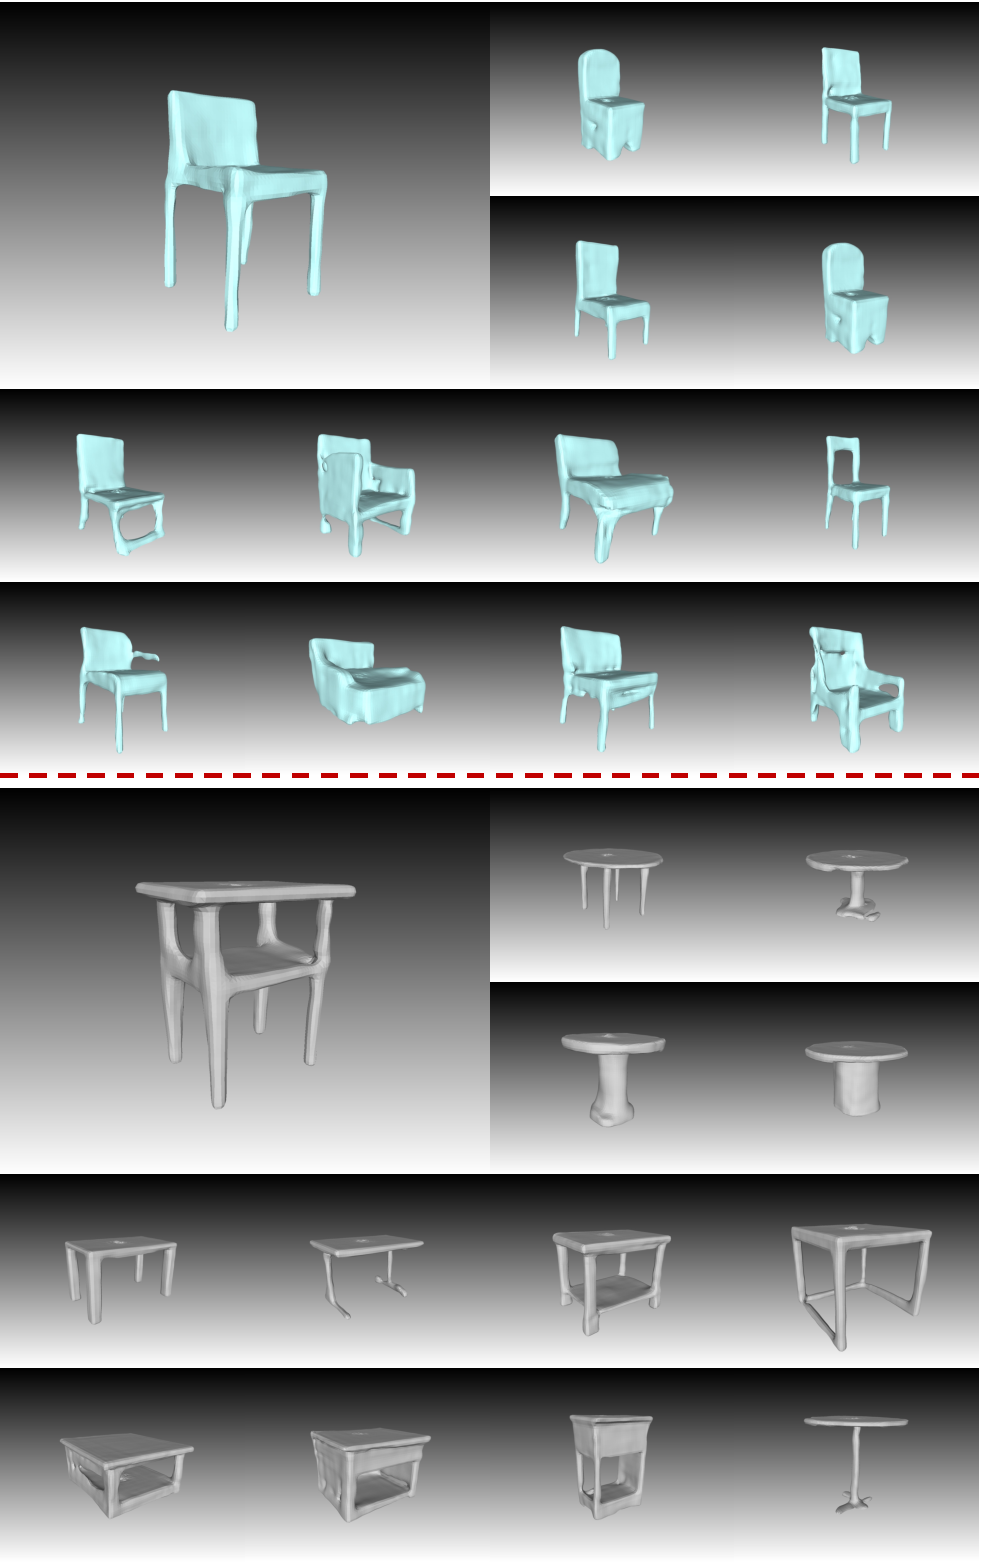
\includegraphics[width=0.85\textwidth]{imgs/table_chair.pdf}
    \caption{Unconditional 3D generation results of table and chair. }
    \label{fig:chairs_table_unconditional} 
\end{figure}

\section{Experiment Details}
所有的实验均在单卡 NVIDIA RTX 4090D 上进行, learning rate scheduler 使用 \texttt{CosineAnnealingLR}, 其中 $\texttt{lr} = 10^{-4}$, $\texttt{eta\_min} = 10^{-6}$. 优化器均为 Adam, 
其他超参数设置见表 \cref{tab:params}.
\begin{table}[htbp]
    \centering
    \begin{tabular}{cccccccc}
        \toprule
        \textbf{Experiments}  &  \textbf{category} & \textbf{batch size} & \textbf{\#epoch} & \textbf{train timesteps}\\ 
        \midrule
        \textbf{VQ-VAE} & \texttt{all} & 8 &  50 & N/A \\
        \midrule
        \multirow{4}{*}{\textbf{Unconditional}}  & \texttt{table} & 12 & 200 & 5000 \\
        & \texttt{chair} & 12 & 200 & 5000 \\
        & \texttt{sofa} & 12 & 200 & 5000 \\
        & \texttt{rifle} & 12 & 400 & 5000\\
        \midrule
        \textbf{Conditional} & \texttt{table, chair} & 40 & 30 & 3000  \\
        \bottomrule
    \end{tabular}
    \caption{The parameters of the experiments. }
    \label{tab:params}
\end{table}

\paragraph{Datasets.} VQ-VAE 的训练数据集为 ShapeNet~\cite{shapenet} 中的 \texttt{chair}, \texttt{rifle}, \texttt{table}, \texttt{sofa} 和 \texttt{speaker} 5类物体, 按照 SDFusion 中的方法划分为训练集与测试集, 详见 \texttt{./dataset\_info\_files/}. 
Unconditional Generation 的针对每个类别单独训练, 得到的模型可以生成对应类别的物体, 实际上也基于 \texttt{speaker}的数据进行了一次训练, 但是由于模型精度问题, 生成的结果基本为一个长方体, 故未在报告中展示. Text Conditioned Generation 的文本描述来自 Text2Shape~\cite{chen2018text2shape} 数据集, 只使用了 \texttt{chair} 和 \texttt{table} 两类物体的描述, 按照 SDFusion 中的方法划分为训练集与测试集.

\begin{figure}[htbp]
    \centering
    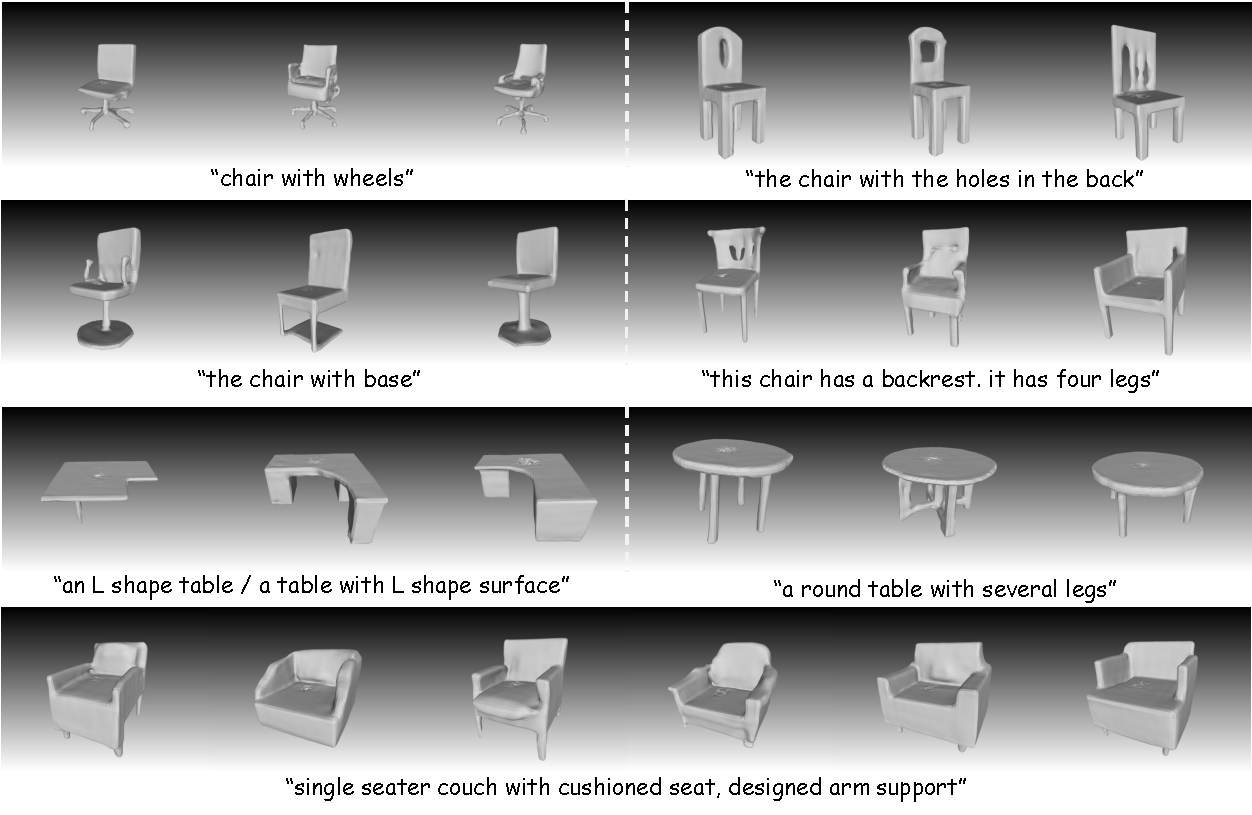
\includegraphics[width=1.0\textwidth]{imgs/result_text_2.pdf}
    \caption{Conditional 3D generation results of table and chair with text prompts.}
    \label{fig:conditional_text_1}
\end{figure}
\vspace{-1em}
\paragraph{测试.}  对于VQ-VAE, 随机从测试集中采样若干 SDF, 得到重建后的结果 (\cref{fig:reconstruction_vqvae}). 对于 Unconditional Generation, 每次随机采样若干个噪声latent. 对于文本条件生成, 
使用了 SDFusion 论文与 supplementary 中的文本描述与自己基于测试集修改的文本描述, 生成的结果见~\cref{fig:conditional_text_1,fig:conditional_text_2}.
在实际测试中, Marching Cubes 的 SDF Threshold 设置在 $[0.001, 0.008]$ 之间, 去噪步数设置在 $[1000, 5000]$ 之间 (注意不能超过模型训练时的最大步数), guidance scale 设置在 $[5, 7.5]$ 之间.
Noise scheduler 使用了 \texttt{diffusers} 库提供的 DDPM 接口, 可以比较方便地替换为其他scheduler.
\section{Results Analysis}
\subsection{Unconditional Generation}
\begin{figure}[htbp]
    \centering
    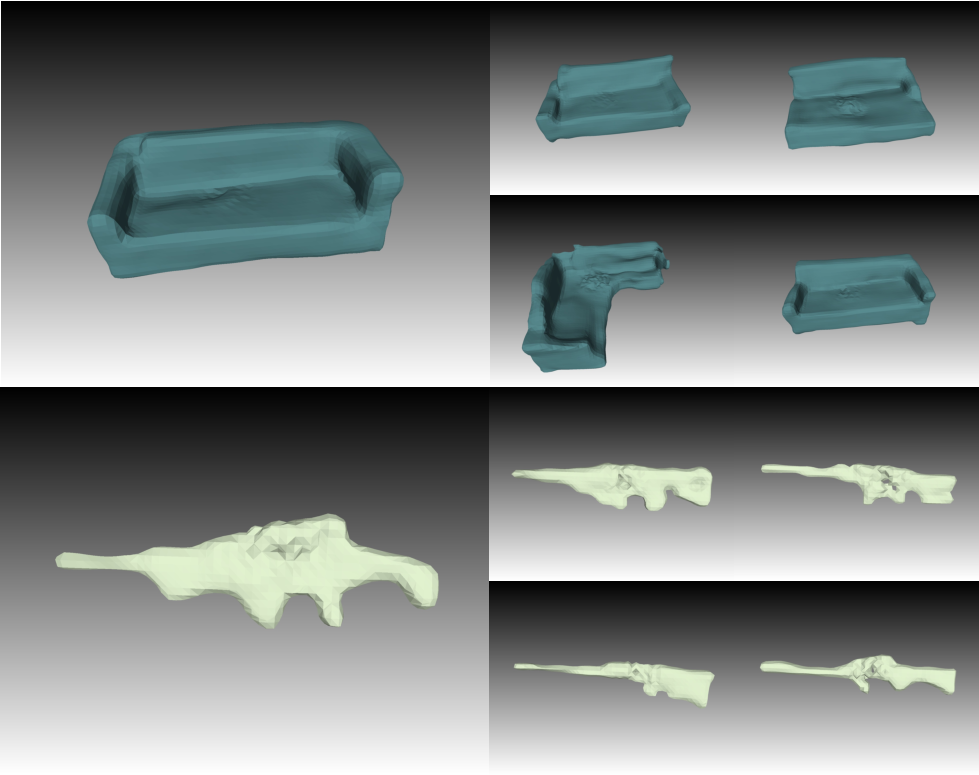
\includegraphics[width=0.8\textwidth]{imgs/sofa_rifle.pdf}
    \caption{More unconditional 3D generation results of sofa and rifle. }
    \label{fig:sofa_rifle_unconditional} 
\end{figure}

Unconditional Generation 的结果见~\cref{fig:chairs_table_unconditional,fig:sofa_rifle_unconditional}, 发现可以生成比较多样的物体形状, 如可以生成各类不同形状的椅子与桌子, 同时几何形状也比较合理.
但细节的生成效果不佳, 例如\texttt{chair} 的腿部细节 (见~\cref{fig:fail}) 及\texttt{rifle} 的整体生成细节 (见~\cref{fig:sofa_rifle_unconditional}) 较差. 一部分可能原因是 VQ-VAE 重建的 SDF 信息损失. 
另一部分可能是由于 \texttt{rifle} 物体较小且相对数据量较小.

\subsection{Text Conditioned Generation}
\cref{fig:conditional_text_1} 中展示了各类文本条件生成的结果, 可以看到模型能够根据文本生成对应的物体形状, 并且能够控制一些生成的细节. 例如, 可以比较精细地控制椅子的腿部细节 (\texttt{ chair with wheels} 和 \texttt{chair with base}), 与桌子的形状 (\texttt{an L shape table} 和 \texttt{a round table with several legs}).
同时生成的物体多样性较高, \cref{fig:conditional_text_2} 中展示了同一文本描述下丰富的生成结果. 在实际测试中也有一些失败的生成结果, 如\texttt{chair with little pillow} 很难生成出小枕头的细节, 主要原因猜测是训练数据中相关的描述较少, 同时由于时间算力原因, 使用了中等大小的模型, 可能无法捕捉到所有细节.

\begin{figure}[htbp]
    \centering 
    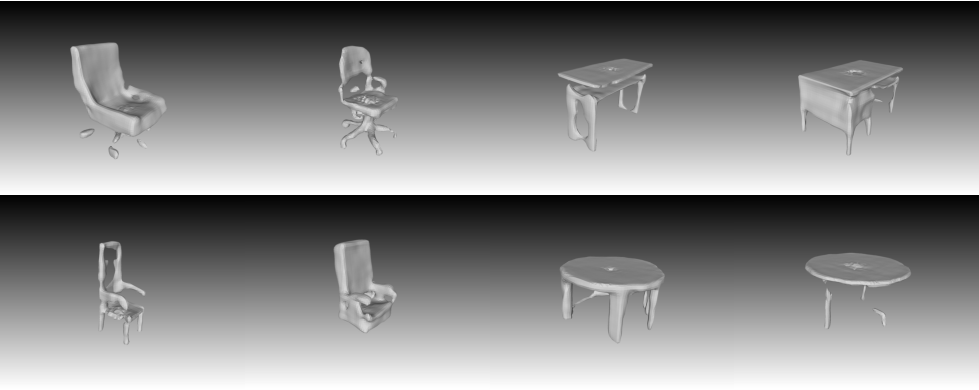
\includegraphics[width=0.85\textwidth]{imgs/fail.pdf}
    \caption{Failure cases of the unconditional generation.}
    \label{fig:fail}
\end{figure}

\begin{figure}[htbp]
    \centering
    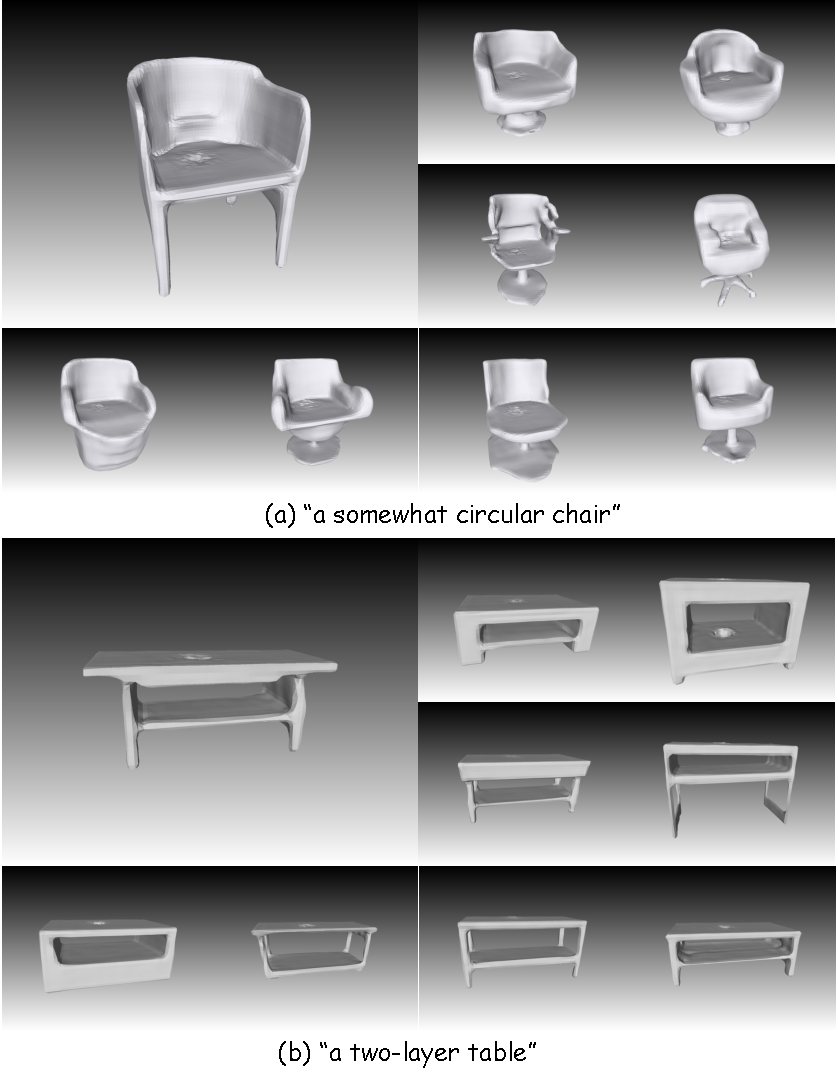
\includegraphics[width=0.75\textwidth]{imgs/result_text_1.pdf}
    \vspace{-1em}
    \caption{More conditional 3D generation results of table and chair with text prompts.}
    \label{fig:conditional_text_2}
\end{figure}



\section{Conclusion}
本项目实现了基于 VQ-VAE 和 Diffusion Model 的 3D 物体生成, 包括无条件生成与文本条件生成. 目前得到的结果能够生成较为多样的物体形状, 在实验过程中发现相较于纯 \texttt{ResidualUNet3D} 模型, 添加了 Attention 模块后, 生成的物体的稳定性相对有所提升.

限于时间关系, 本项目没有尝试尝试实现 image-to-3D 的生成 (实际感觉上和文本条件生成类似, 使用一个预训练的图像编码器后, 训练 U-Net 即可). 同时没来得及尝试 texture generation/style transfer 的部分, 可以在之后的空闲时间中继续探索.

此外比较奇怪的是, 3D Diffusion Model 的开源代码尚未像 image Diffusion Model 有一个统一且活跃的代码库(\texttt{diffusers}), 也许是我了解的不多.

\section*{Acknowledgements}
感谢王鹏帅老师和助教们一学期的付出, 这是我所上的第一门图形学/三维视觉相关课程, 受益匪浅. 
感谢 SDFusion, pytorch-3dunet, diffusers 等开源项目的作者们和社区贡献者们, 
此外也感谢 VS Code Copilot(Claude Sonnet 4) 陪伴我一起 coding and debug :<). 

\bibliographystyle{plain} 
\bibliography{ref} 

\end{document}